\section{Experiences with Hadoop}
\label{sec:hadoop}

We experimented with Hadoop on our cluster to confirm and better
understand the inefficiency exposed by our analysis of reported
benchmark results.
%and Section~\ref{sec:benchmarks}, we also measured the speed of Hadoop
%sorts on our cluster for up to 100 GB over 25 nodes.  We use weak
%scaling by keeping the amount of data per node constant and increasing
%the total amount of data to be sorted along with the active cluster size.


\minorsection{Tuning Hadoop's settings} Default Hadoop settings fail
to use most nodes in a cluster, using only two (total) map tasks and
one reduce task.  Even increasing those values to use four map and
reduce tasks per node, a better number for our cluster, with no
replication, still results in lower-than-expected performance.  We improved
the Hadoop sort performance by an additional 2$\times$ by adjusting a
number of configuration settings as suggested by Hadoop cluster setup
documentation and other
sources~\cite{hadoopsetup,hadoopsetup2,hadoopsetup3}.
%Initially we started with the
%default Hadoop settings, but by adjusting some key configurations we
%were able to improve sort times by a large factor. The actual number
%of possible settings and values were too large to do an exhaustive
%search, so there are certainly better settings and more changes to
%improve these Hadoop results even further.  However, these results
%represent our best efforts to adjust settings in ways commonly
Table~\ref{table:hadoop:settings} describes our changes, which
include reducing the replication level, increasing block sizes,
increasing the numbers of map and reduce tasks per node, and increasing
heap and buffer sizes.
%settings we changed to improve Hadoop's performance on our cluster,
%where one disk per node was made available to HDFS and up to 25 slave
%nodes (and one dedicated NameNode) were used for our experiments.
%First we changed the replication level from 3 to 1, to focus on the
%fastest case where replication is not necessary.  Larger block sizes
%helped our reads and writes go faster, and amortized the overhead for
%starting each map task.  We increased the maximum number of map and
%reduce tasks run in parallel per node, since our machines could handle
%the increased load.  We also increased the Java VM heap size, the
%Hadoop daemon heap size (used by each NameNode/DataNode and
%JobTracker/TaskTracker), the memory buffer sizes used for sorting, and
%the number of streams merged together when sorting.

Interestingly, we found that speculative execution did not improve
performance for our cluster.
Occasional map task failures and lagging nodes can
and do occur, especially when running over more nodes.
However, they are less common for our smaller cluster size
(one NameNode and 1--25 slave nodes), and surprisingly they
had little effect on the overall performance when they did occur.
%Add speculative execution citation from LATE paper in OSDI08?
When using speculative execution, it is generally
advised to set the number of total reduce tasks to 95---99\% of the
cluster's reduce capacity to allow for a node to fail and still
finish execution in a single wave.  Since failures are less of an
issue for our experiments, we optimized for the failure-free case and
chose enough Map and Reduce tasks for each job to fill every machine
at 100\% capacity.

{
\renewcommand{\baselinestretch}{1.0}
\begin{table}
\centering
\begin{minipage}{1\textwidth}
\centering
\renewcommand{\arraystretch}{1.2}
\begin{tabular}{|p{3.0cm}|c|c|p{9.4cm}|}
\hline
Hadoop Setting & Default & Tuned & Effect \\ \hline
Replication level & 3 & 1 & The replication level was set to 1 to
avoid extra disk writes. \\ \hline
HDFS block size & 64 MB & 128 MB & Larger block sizes in HDFS make large file reads and writes faster, amortizing the overhead for starting each map task. \\ \hline
Speculative exec. & $true$ & $false$ & Failures are uncommon on small clusters, avoid extra work. \\ \hline
Maximum map tasks per node  & 2 & 4 & Our nodes can handle more map
tasks in parallel. \\ \hline
Maximum reduce tasks per node & 1 & 4 & Our nodes can handle more
reduce tasks in parallel. \\ \hline
Map tasks & 2 & $4n$ & For a cluster of $n$ nodes, maximize the map tasks per node. \\ \hline
Reduce tasks & 1 & $4n$ & For a cluster of $n$ nodes, maximize the reduce tasks per node. \\ \hline
Java VM heap size & 200 MB & 1 GB & Increase the Java VM heap size for each child task. \\ \hline
Daemon heap size & 1 GB & 2 GB & Increase the heap size for Hadoop daemons. \\ \hline
Sort buffer memory & 100 MB & 600 MB & Use more buffer memory when sorting files.  \\ \hline
Sort streams factor & 10 & 30 & Merge more streams at once when sorting files. \\ \hline
\end{tabular}
\caption{Hadoop configuration settings used in our experiments.
%By tuning these Hadoop settings on our smaller cluster and running the specified maximum number of map and reduce tasks per node, our Hadoop sort benchmark completed about twice as fast as with the default Hadoop settings. While the actual default settings use 2 map tasks and 1 reduce task, that wouldn't actually make use of the full cluster of available machines.  Therefore, our modified default settings used a replication level of 1, $2n$ map tasks and $n$ reduce tasks.}
}
\label{table:hadoop:settings}
\end{minipage}
\end{table}
}


\minorsection{Sort measurements and comparison to the model}
\label{sec:hadoop:results}
Figure~\ref{fig:hadoopsort} shows sort results for different numbers
of nodes using our tuned Hadoop configuration.  Each measurement sorts
4~GB of data per node (up to 100~GB total over 25~nodes).  Random
100~byte input records were generated with the \emph{TeraGen} program,
spread across active nodes via HDFS, and sorted with the standard
\emph{TeraSort} Hadoop program.  Before every sort, the buffer cache
was flushed (with \texttt{sync}) to prevent previously cached writes
from interfering with the measurement.  Additionally, the buffer cache
was dropped from the kernel to force disk read operations for the
input data.  The sorted output is written to the file system, but not
synced to disk before completion is reported; thus, the reported
results are a conservative reflection of actual Hadoop sort execution
times.

{
\renewcommand{\baselinestretch}{1.0}
\begin{figure}[t]
\begin{center}
\subfigure[Scaling a Hadoop sort benchmark up to 25 nodes.]{
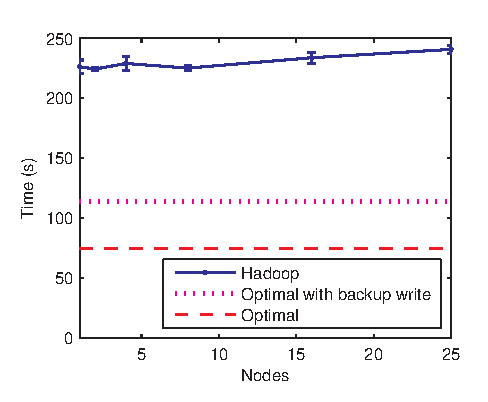
\includegraphics{fig_hadoop_sort.eps}
\label{fig:hadoopsort:scale}
}
\subfigure[Time breakdown into phases.]{
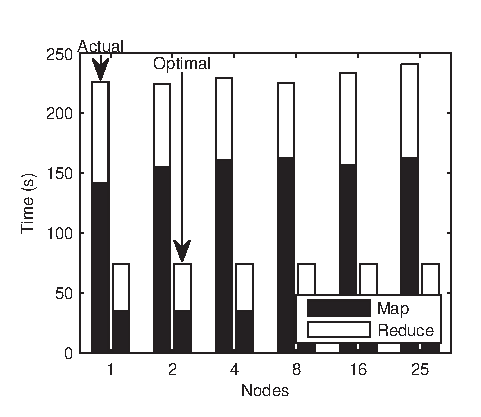
\includegraphics{fig_hadoop_breakdown.eps}
\label{fig:hadoopsort:breakdown}
}

\minicaption{Measured and optimal sort runtimes for a tuned Hadoop
  cluster.  Performance is about 3 times slower than optimal, and 2
  times slower than an optimal sort that includes an extra backup
  write for the map output, which is currently Hadoop's behavior}             
  {Hadoop scales well with 4~GB per node up to 25 nodes, but it is
  inefficient.  The measured runtime, optimal calculation, and optimal with
  backup write calculation are shown in {\bf (a)}.  The breakdown of
  runtime into map and reduce phases is shown in {\bf (b)}.

  % shows that a majority is spent in the map
  %, but there is considerable overhead
  %for creating and managing map and reduce tasks.  A breakdown
  %of the time in {\bf (b)} shows that a majority is spent in the map
  %phase, which includes time to setup the map and reduce tasks,
  %perform the map operation, and transfer data over the network to
  %the appropriate reducer. The reduce time includes the
  %actual sort and reduce operations, which will write the sorted data locally.}
}
\label{fig:hadoopsort}
\end{center}
\end{figure}
}



The results confirm that Hadoop scales well, since the average runtime
only increases 6\% (14 seconds) from 1 node up to 25 nodes (as the workload
increases in proportion).
For comparison, we also include the optimal sort times in
Figure~\ref{fig:hadoopsort}, calculated from our performance model.
The model's optimal values reveal a large constant inefficiency
for the tuned Hadoop setup---each sort requires 3$\times$ the optimal
runtime to complete, even without syncing the output data to disk.
%starting and managing map and reduce tasks is significant
%- 2 times longer than the predicted optimal times with an intermediate
%backup write, and 3 times longer without the backup write, which is
%unnecessary for our cluster.  If we hadn't tuned Hadoop beforehand,
%but instead used the default settings while being smart to maximize
%the number of map and reduce tasks per node and turn off replication,
%we discovered that it would have taken twice as long.  Put another
%way, tuning our Hadoop cluster from its default settings effectively
%doubled the efficiency of our cluster, but the sort still took 2 to 3
%times longer than an ideal system.

The 6\% higher total runtime at 25 nodes is due to skew in the completion
times of the nodes---this is the source of the $\sim$9\% additional
inefficiency at 25 nodes.
The inefficiency due to OS abstractions is already accounted for, as
discussed in Section~\ref{sec:measure}.
One potential explanation for part of the inefficiency is that Hadoop
uses a backup write for the map output, even though the runtimes are
short enough to make it of questionable merit.
As shown by the dotted
line in Figure~\ref{fig:hadoopsort}a, using the model equation with
a backup write would yield an optimal runtime that is 39~seconds longer.
This would explain approximately 25\% of the inefficiency.
However, as with the sort output, the backup write is sent to the file
system but not synced to disk---with 4~GB of map output per node
and 16~GB of memory per node, most of the backup write data may not
actually be written to disk during the map phase.
It is unclear what fraction of the potential 25\% is actually
explained by Hadoop's use of a backup write.

Another possible source of inefficiency could be unbalanced 
distribution of the input data or the reduce data.
%In terms of the actual workload matching up with the ideal of the
%model
However, we found that the input data is spread almost evenly across the
cluster.
Also, the difference between the ideal split of data and what is
actually sent to each reduce node is less than 3\%.
Therefore, the random input generation along with TeraSort's sampling and
splitting algorithms is partitioning work evenly,
and the workload distribution is not to blame
for the loss of efficiency.

Another potential source of inefficiency could be poor scheduling and task
assignment by Hadoop.
However, Hadoop actually did a good job at scheduling map tasks to run
on the nodes that store the data, allowing local disk access (rather
than network transfers) for over 95\% of the input data.
%The runs
%that had a higher percentage of local tasks was correlated with
%relatively shorter sort times, since less data had to be transferred
%over the network before it was processed.
The fact that this value was below 100\% is due to skew of
completion times where some nodes finish processing their local tasks
a little faster than others, and take over some of the load from the
slower nodes.

We do not yet have a full explanation for Hadoop's inefficiency.
Although we have not been able to verify in the complex Hadoop code,
some of the inefficiency appears to be caused by insufficiently pipelined
parallelism between operators, causing serialization of activities
(e.g., input read, CPU processing, and network write) that should
ideally proceed in parallel.
Part of the inefficiency is commonly attributed to CPU overhead
induced by Hadoop's Java-based implementation.
%Throughout each sort, each core running a map task was pegged at 100\%,
%despite the high-performance CPUs and low-CPU I/O-intensive task
%(reading and partitioning the data).
Of course, Hadoop may also not be using I/O resources at full efficiency.
More diagnosing of Hadoop's inefficiency is a topic for continuing
research.

